\documentclass{article}
\usepackage[utf8]{inputenc}
\usepackage{graphicx}


\title{Cara Menambahkan aplikasi di apex oracle}
\author{Ryan Situmorang }
\date{October 2019}

\begin{document}

\maketitle

\section{Pembuatan Aplikasi}

\begin{enumerate}
    \item langkah pertama dalam pembuatan aplikasi baru di apex online melalui excel adalah dengan membuat sebuah data yang akan kita masukan kedalam apex oracle online. Data yang akan di masukkan sesuai data yang telah di buat contohnya saya memasukkan data Mahasiswa D4 Teknik Informatika 2018 setelah itu buat isi dari atribut yang ada didalam table mahasiswa
    \ref{excel}
    \begin{center}
         \centering
            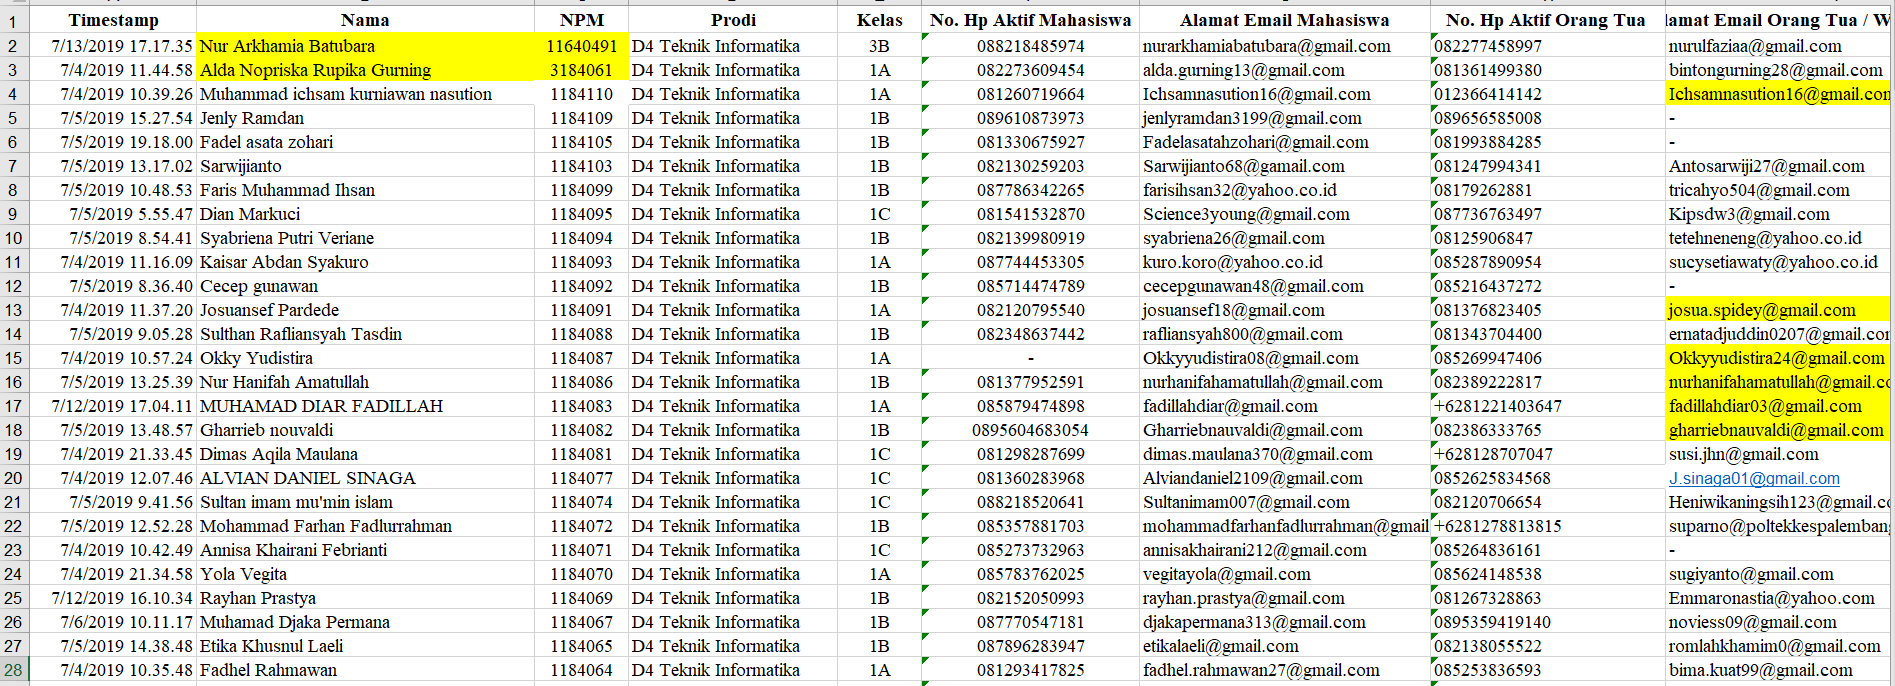
\includegraphics[scale=0.27]{figures/DB0.png}
        \caption{Menambahkan Data}
        \label{excel}
    \end{center}
       
     \item langkah selanjutnya buka di browser apex oracle online setelah itu klik create untuk membuat sebuah aplikasi yang diinginkan
      \ref{create}
    \begin{center}
         \centering
            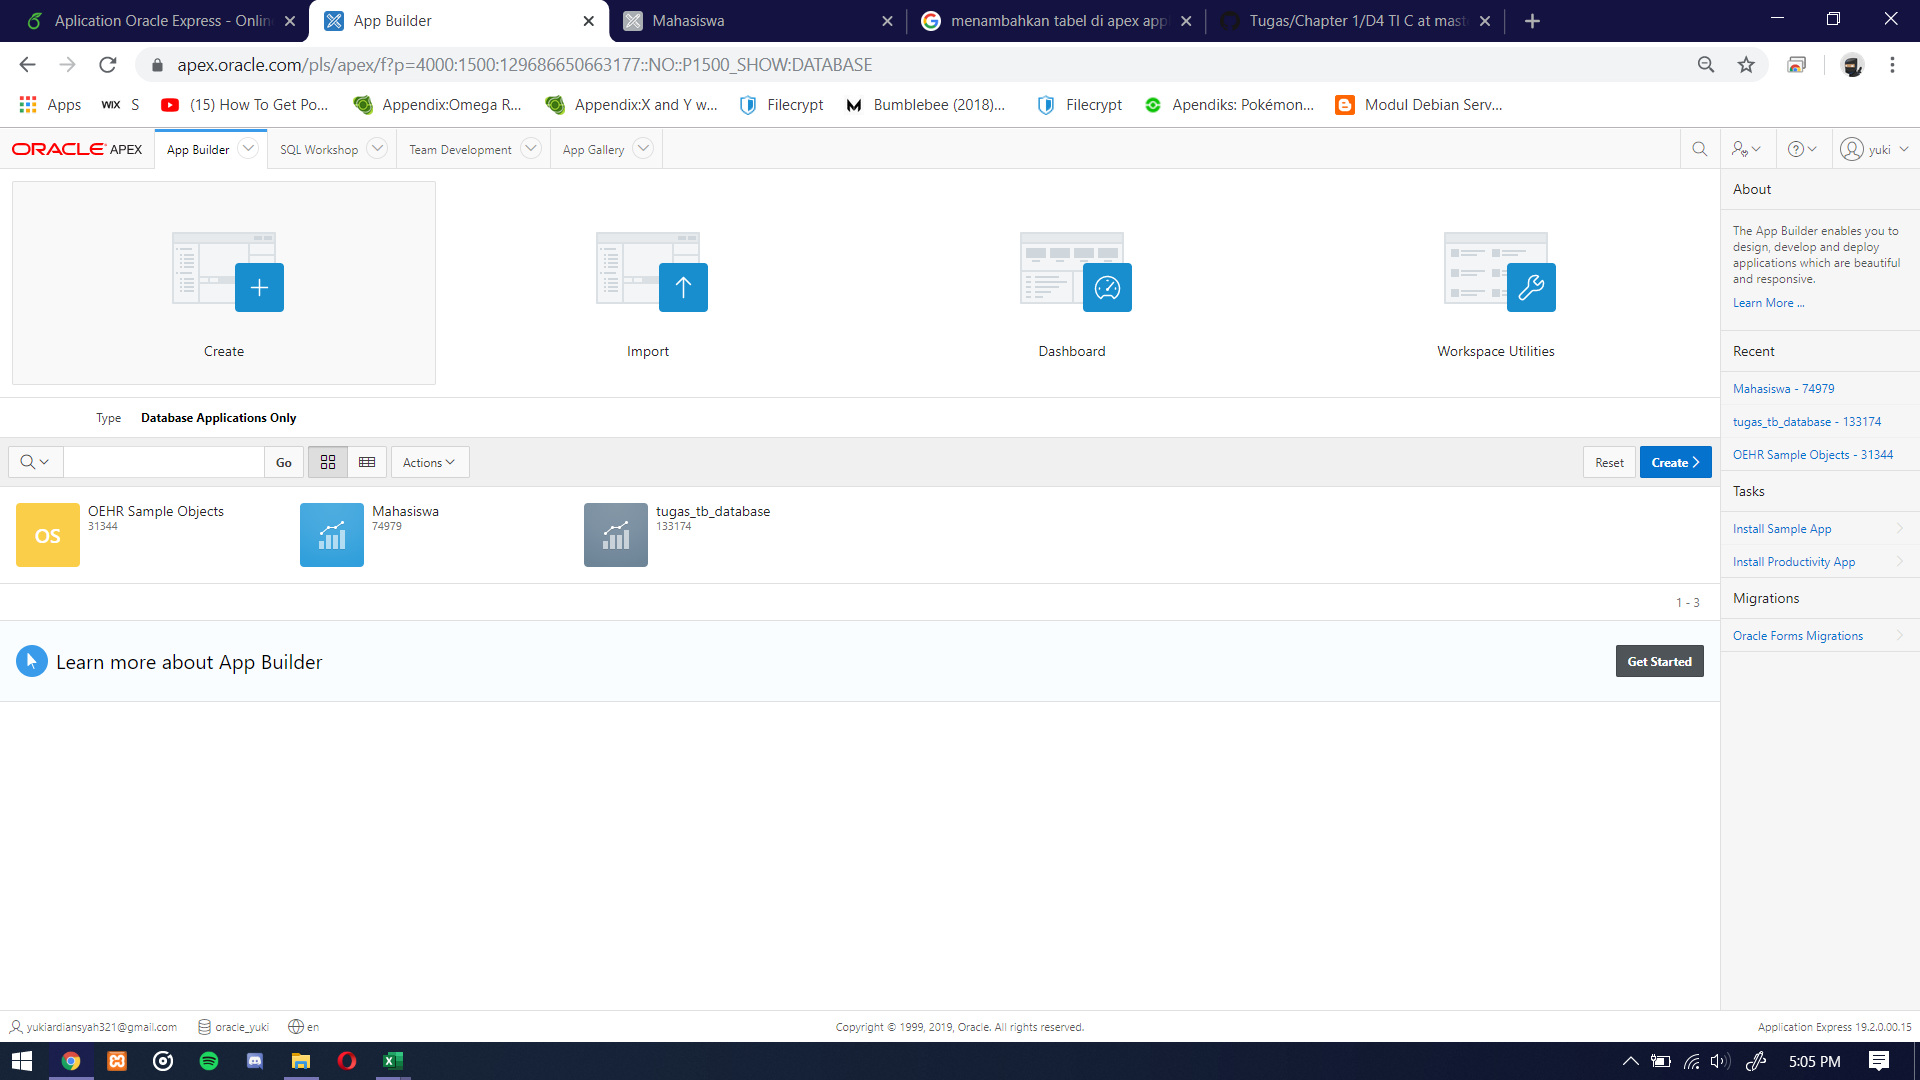
\includegraphics[scale=0.27]{figures/DB1.png}
        \caption{create aplikasi}
        \label{create}
    \end{center}
    
      \item Setelah mengklik create kita melihat 3 cara menambahkan data dalam aplikasi yang ingin di buat klik from a file agar dapat memilih file excel yang telah dibuat
      \ref{from}
    \begin{center}
         \centering
            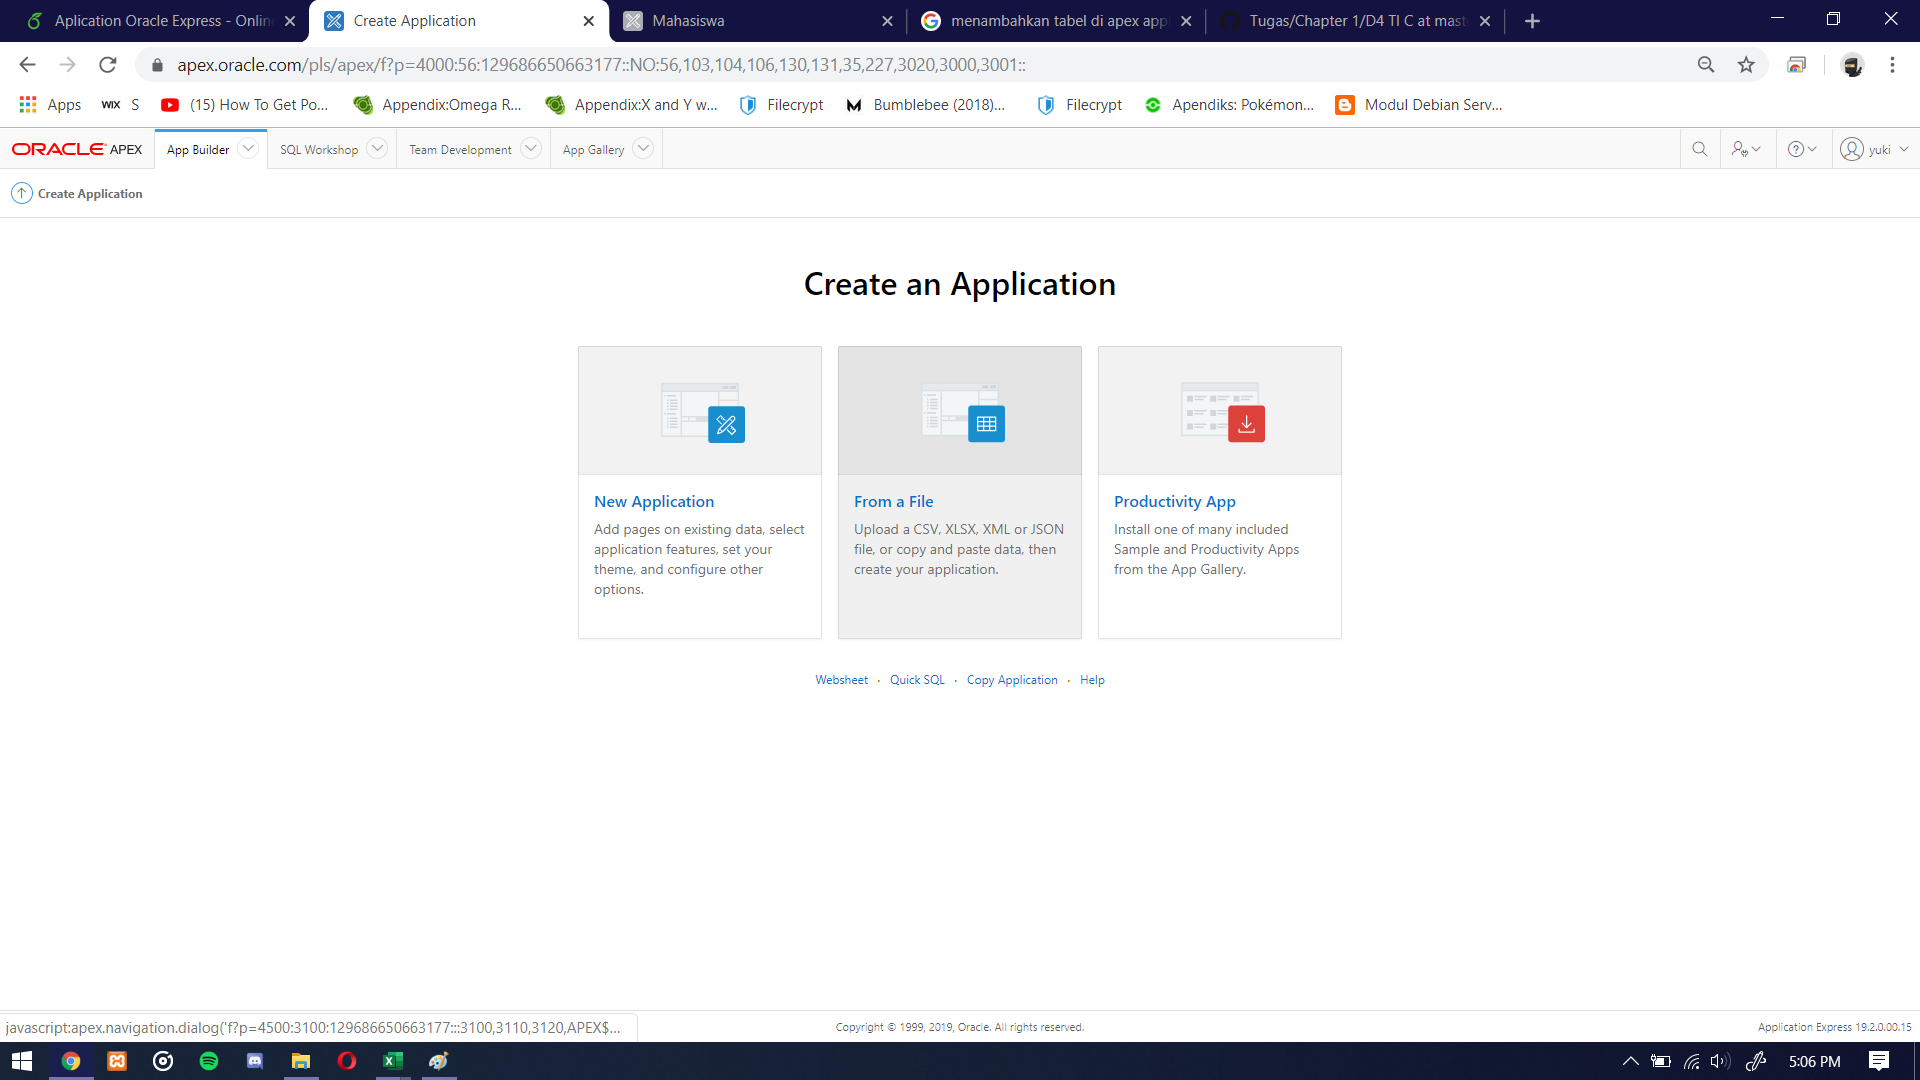
\includegraphics[scale=0.27]{figures/DB2.png}
        \caption{chosse a file}
        \label{from}
    \end{center}
    
    \item Setelah mengklik pilihan from a file system akan menampilkan load data yang berguna untuk memilih jenis file apa yang akan direlafikasi menjadi sebuah table. klik chosse file from a computer untuk memilih file excel yang telah di buat
      \ref{chosse}
    \begin{center}
         \centering
            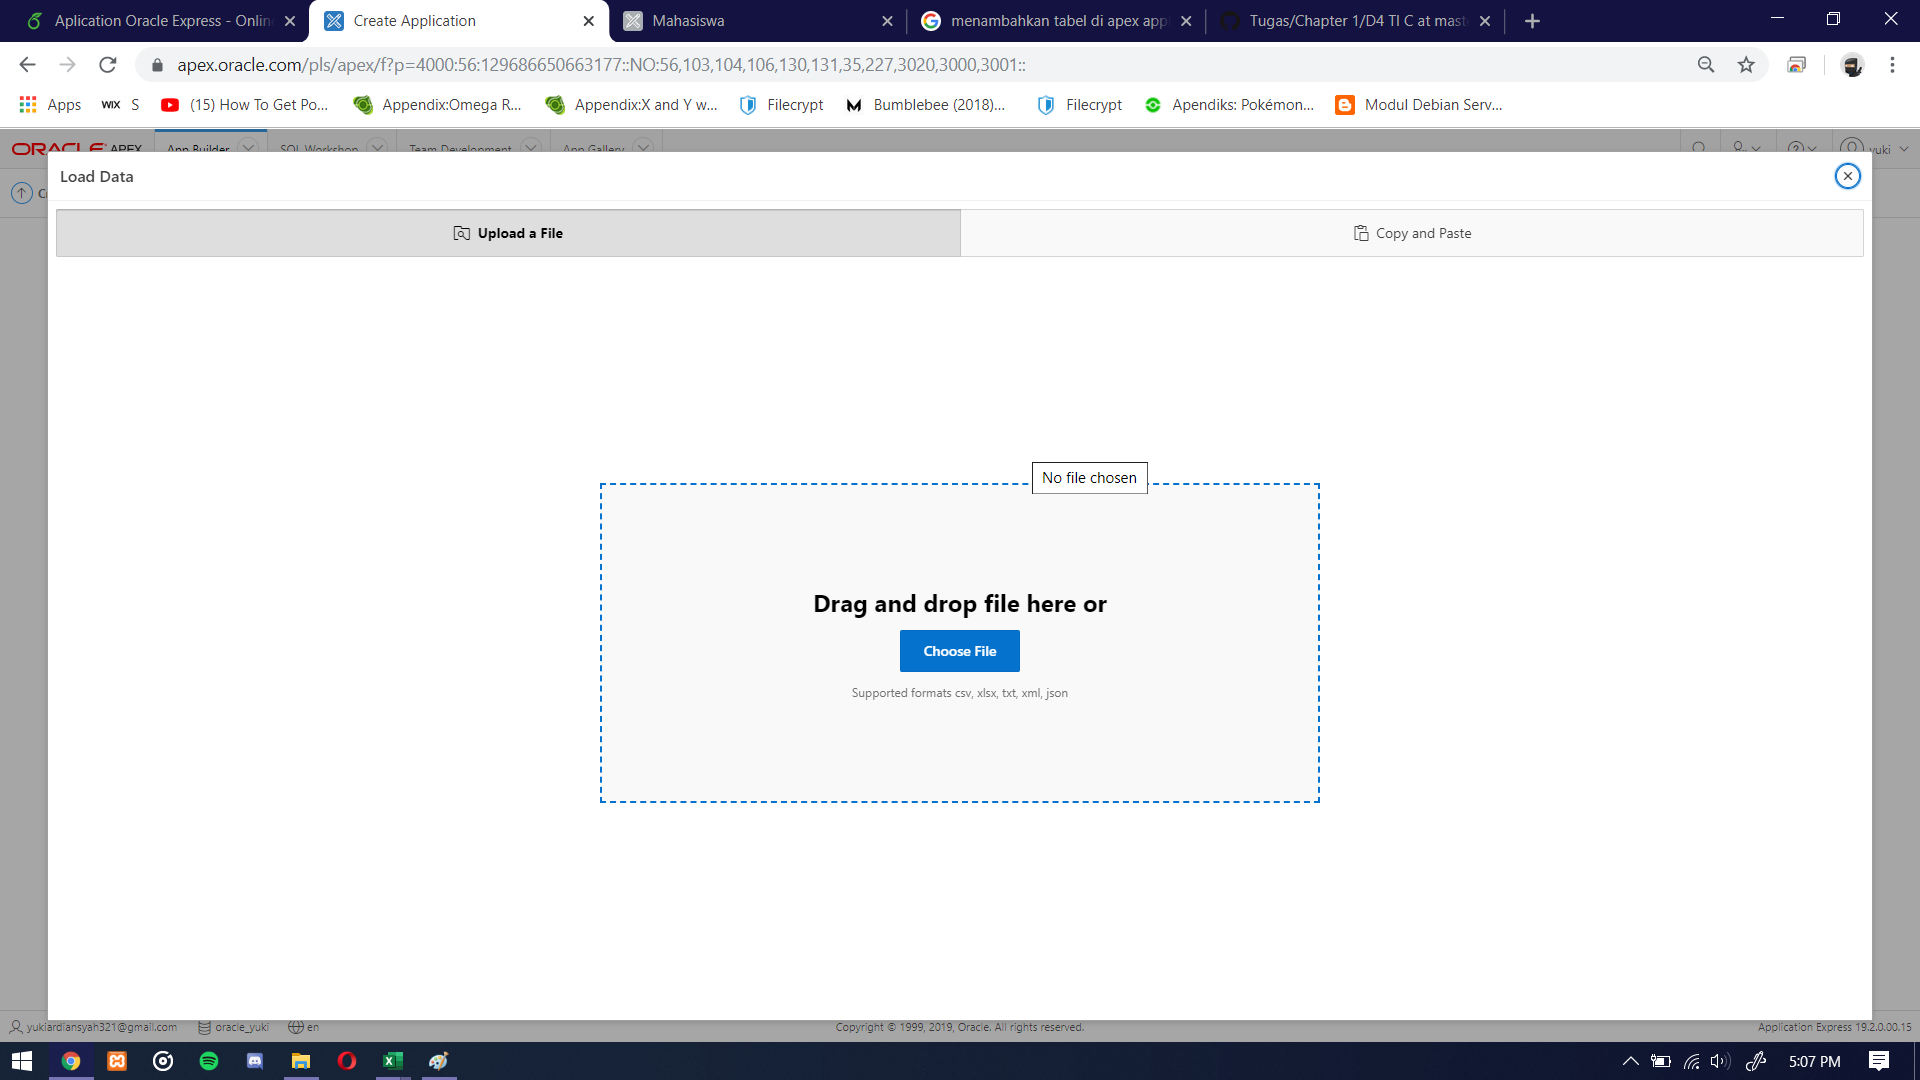
\includegraphics[scale=0.27]{figures/DB3.png}
        \caption{LOAD DATA}
        \label{chosse}
    \end{center}
    
     \item Namai table sesuai dengan data yang kita buat contoh mahasiswa setelah itu klik load data dan tunggu proses selanjutnya
      \ref{excel}
    \begin{center}
         \centering
            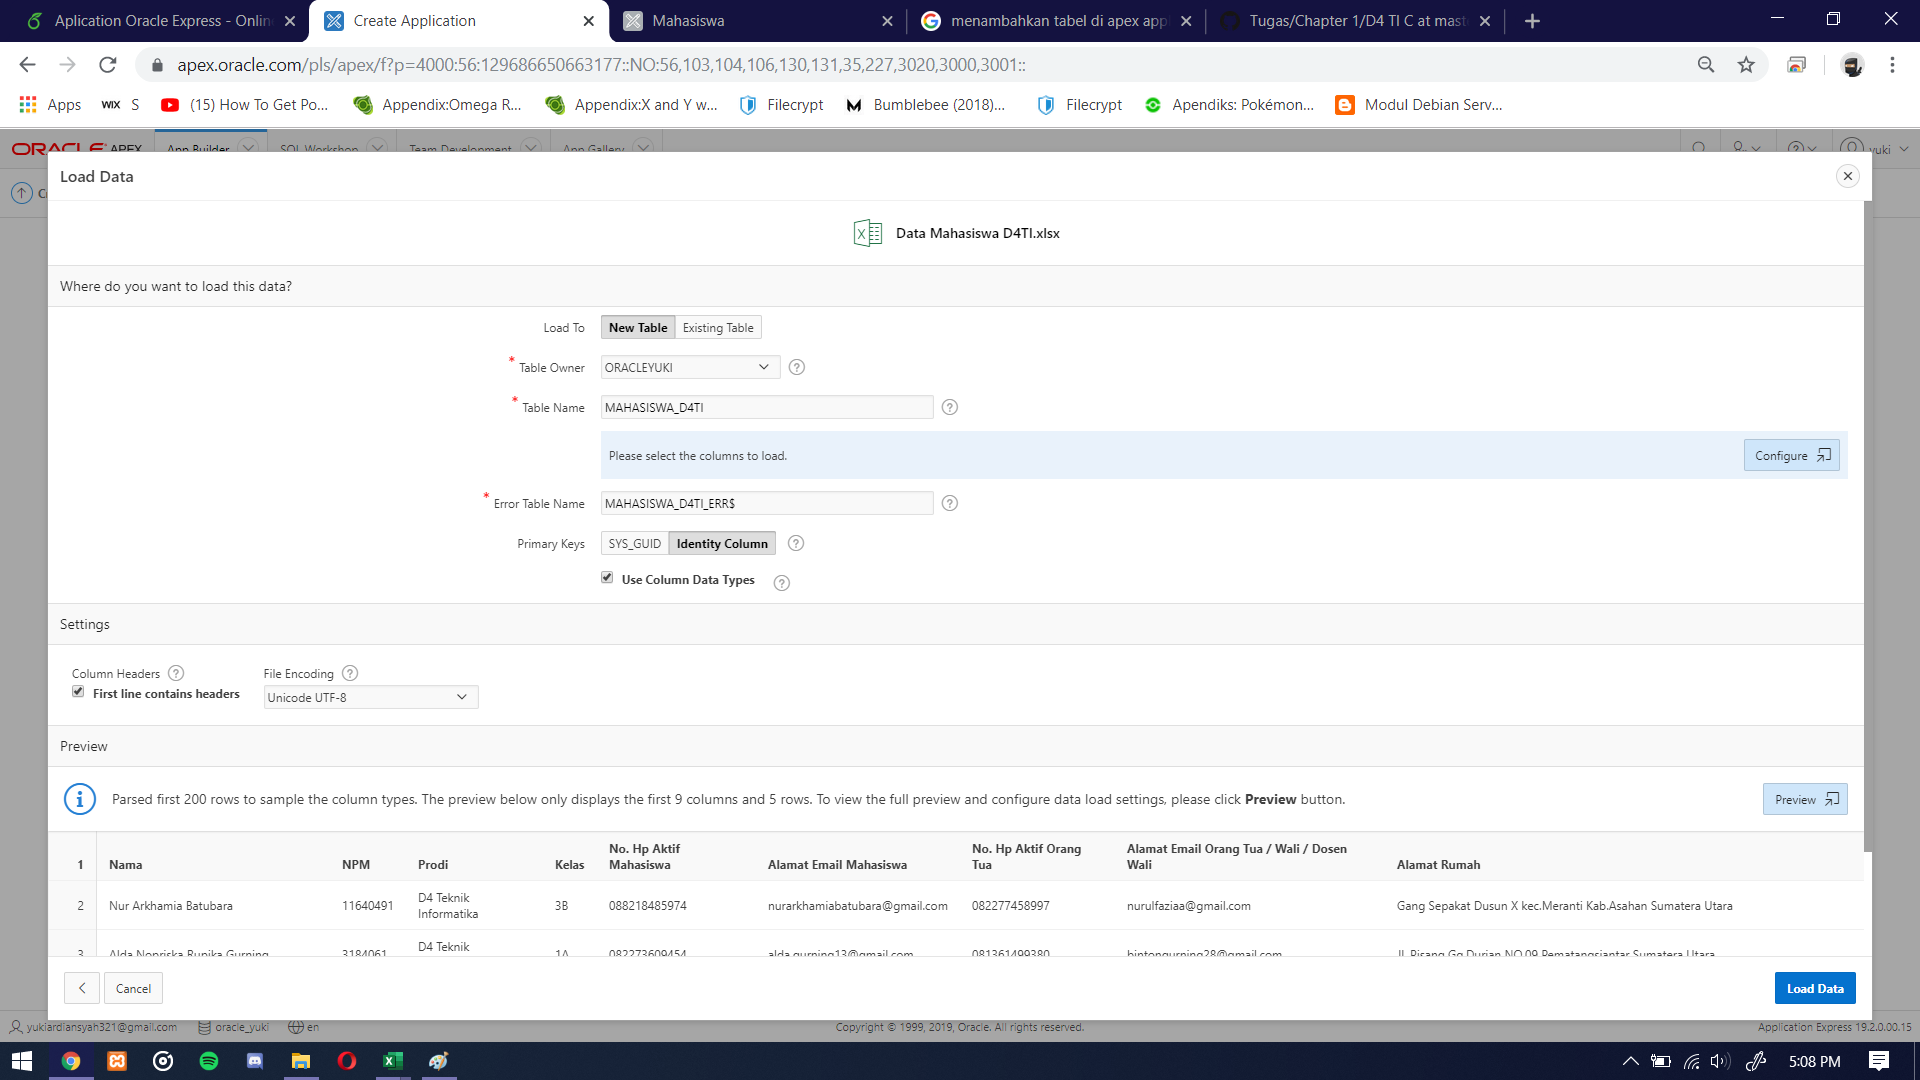
\includegraphics[scale=0.27]{figures/DB4.png}
        \caption{Drag and Drop}
        \label{excel}
    \end{center}
    
     \item setelah itu klik create aplications dan tunggu sampai proses pembuatan report dari aplikasi selasai
      \ref{excel}
    \begin{center}
         \centering
            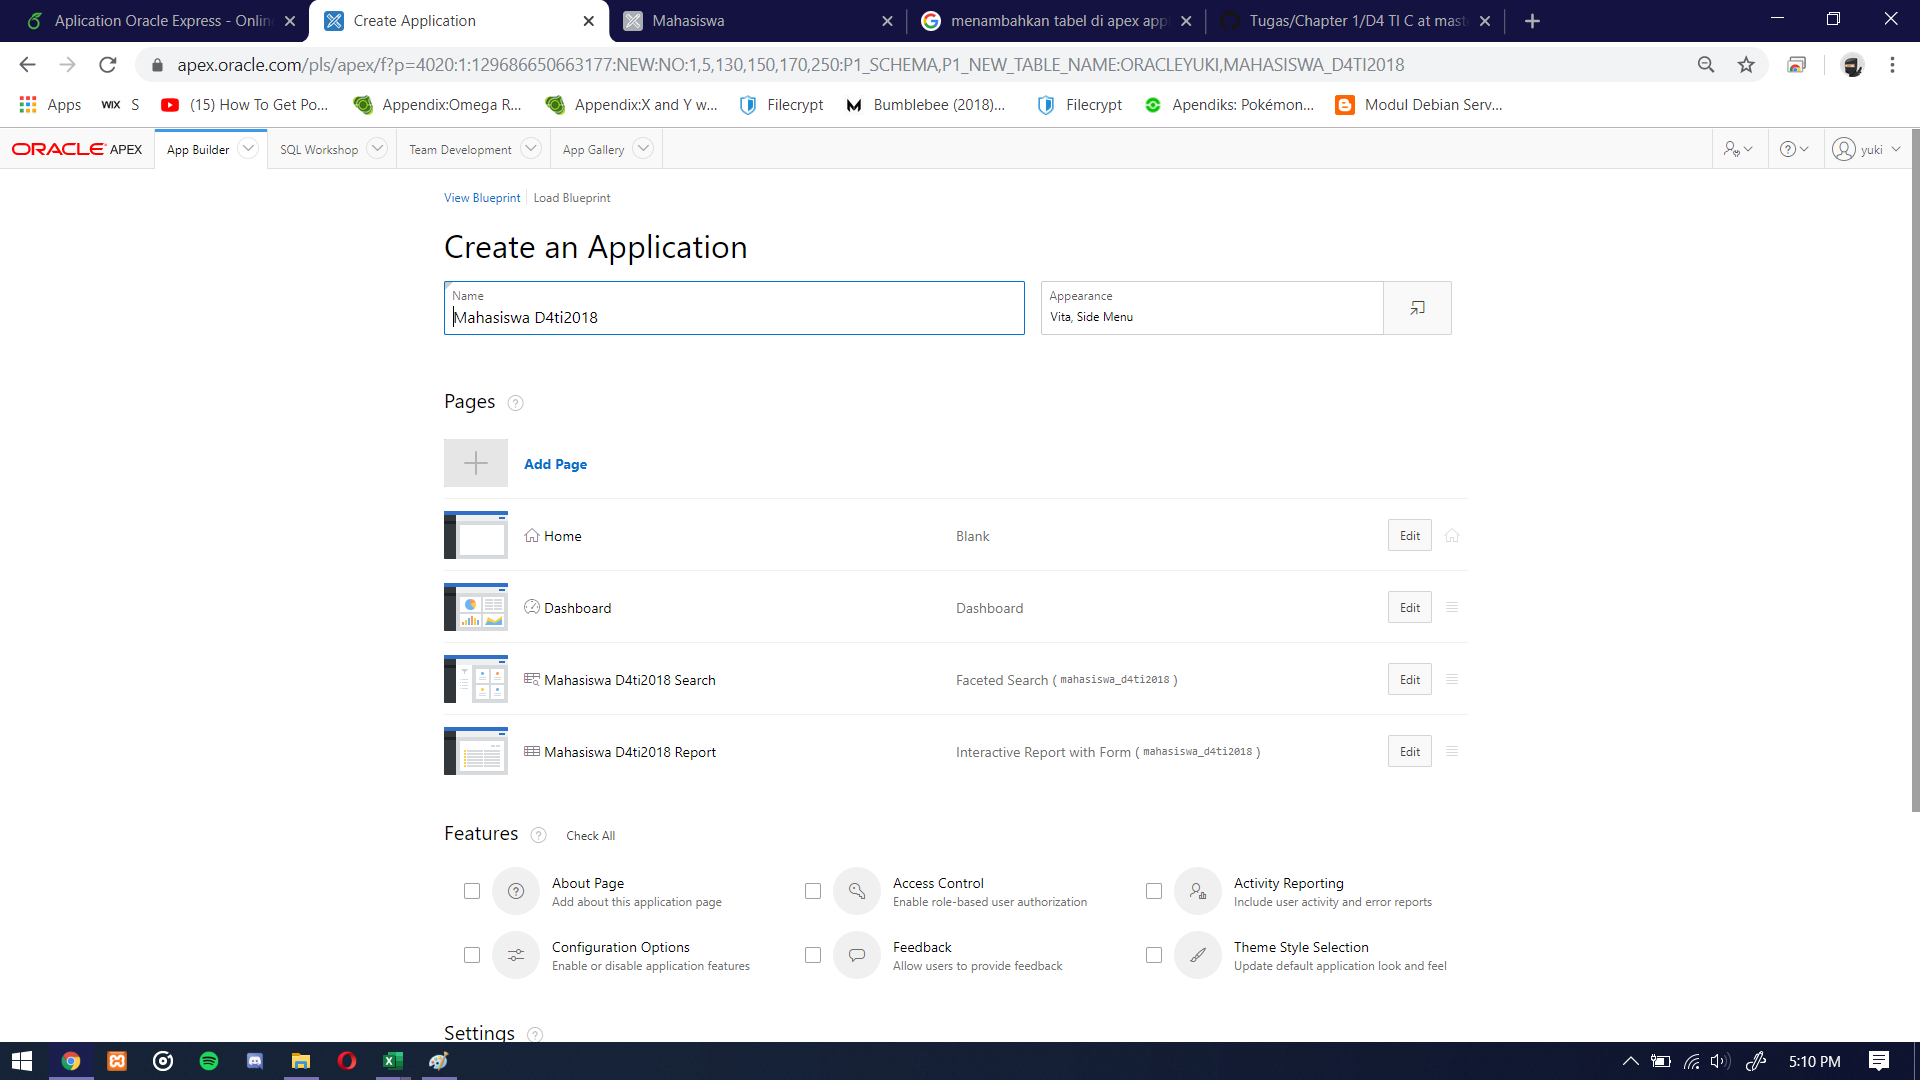
\includegraphics[scale=0.27]{figures/DB5.png}
        \caption{proses create aplication}
        \label{excel}
    \end{center}
    
     \item setelah proses create report selesai kli run aplication untuk menjalankan data yang telah dibuat
      \ref{excel}
    \begin{center}
         \centering
            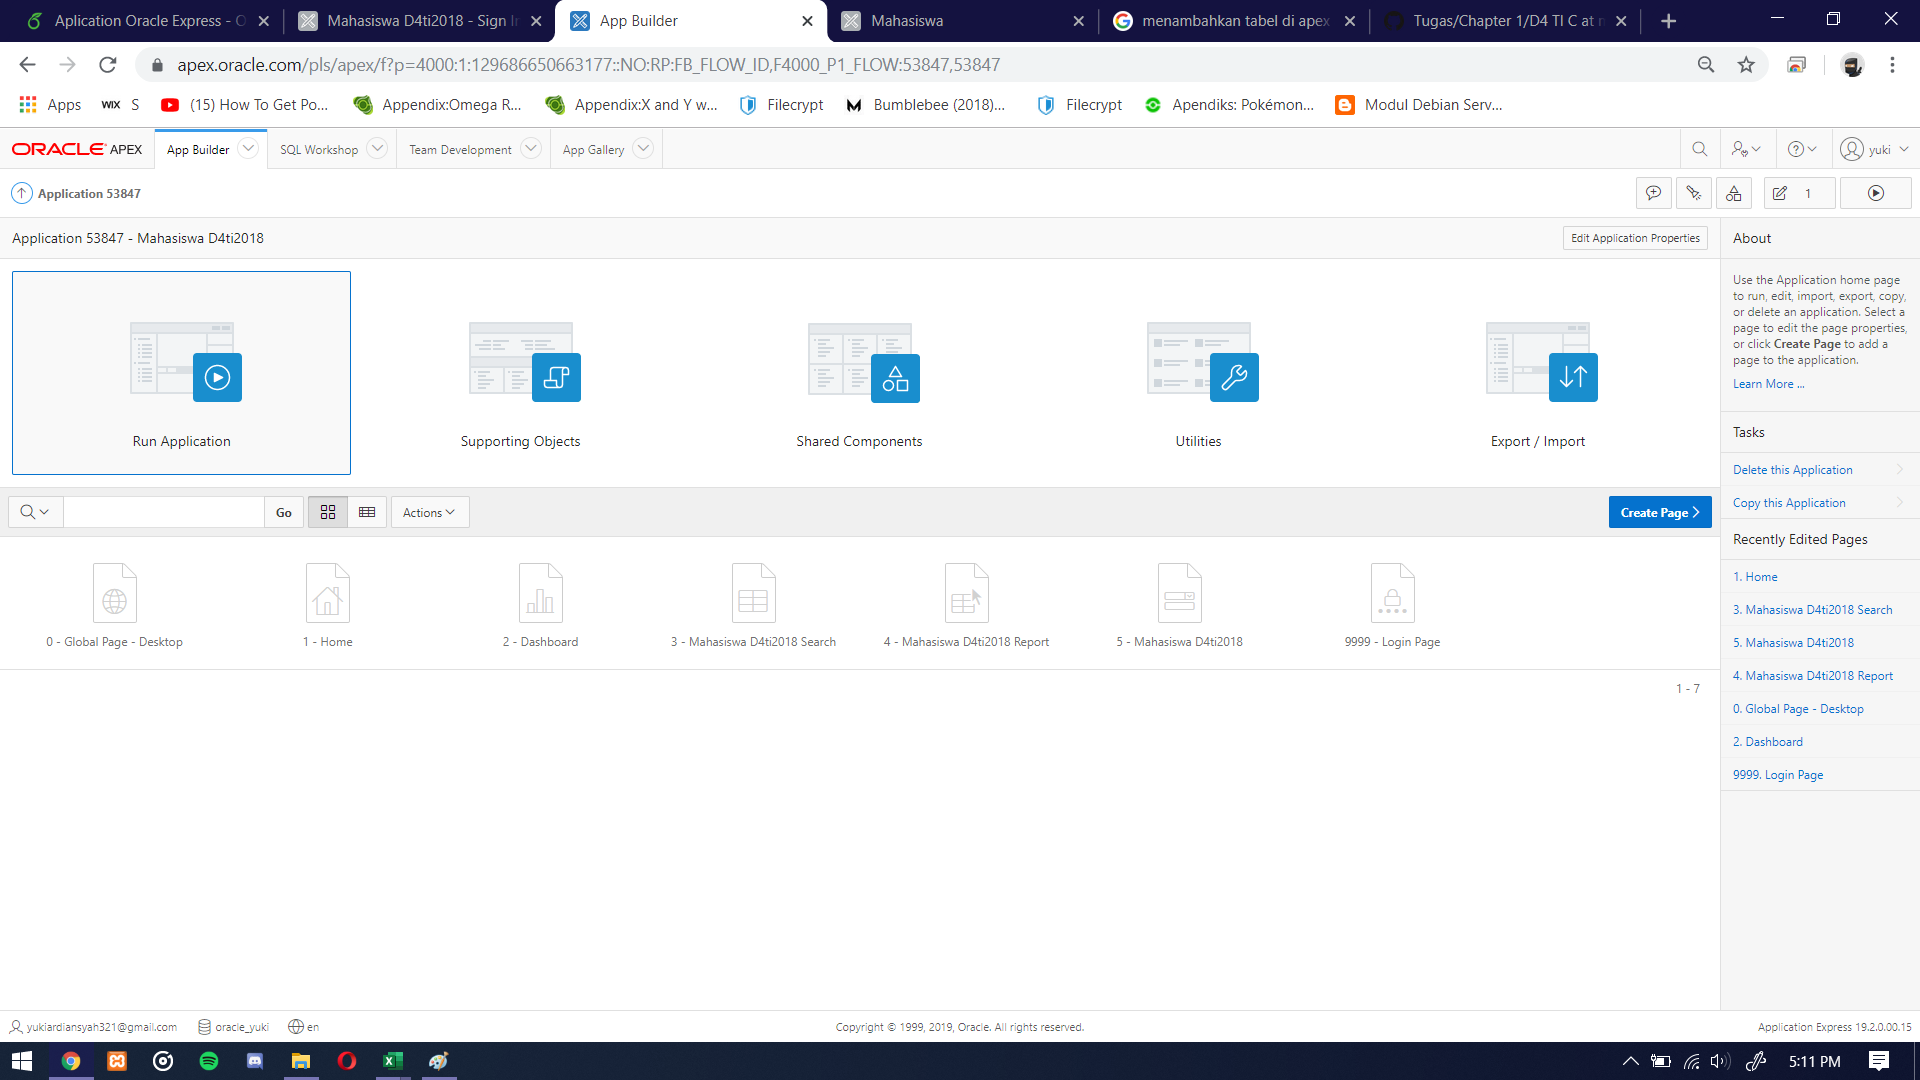
\includegraphics[scale=0.27]{figures/DB6.png}
        \caption{run aplication}
        \label{excel}
    \end{center}
    
      \item Masukkan paswword dan username dari aplikasi apex oracle online untuk membuka aplikasi yang telah dibuat dan untuk melihat hasilnya
      \ref{excel}
    \begin{center}
         \centering
            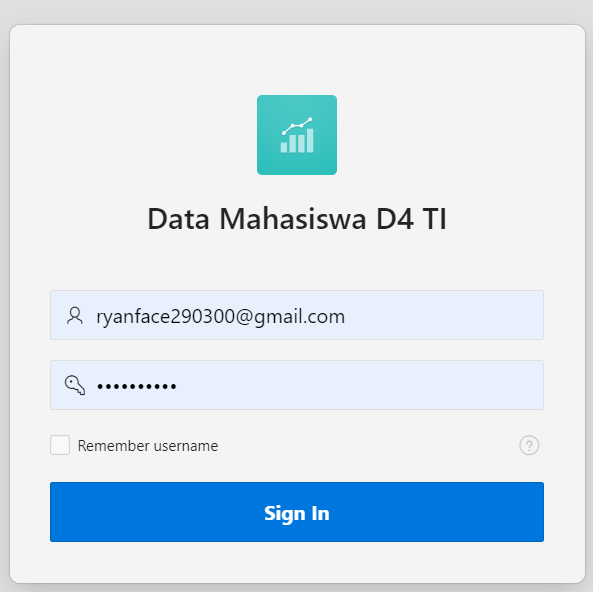
\includegraphics[scale=0.27]{figures/DB7.png}
        \caption{password}
        \label{excel}
    \end{center}
    
\end{enumerate}

\section{Password username}
      
      \begin{enumerate}
          \item workspace "ORACLE(underscore)RY"
          
          \item username "ryanface290300@gmail.com "
          
          \item password "Situmorang"
      \end{enumerate}
      
       

\end{document}
